%%
\chapter{Metoda zrealizowania pracy}
\begin{quotation}
%%
\indent Realizacja pracy opiera się na opracowaniu kroków, które należy podjąć aby stworzyć świat gry w stylu low-poly. Aby zaprezentować stworzone elementy, został stworzony projekt gry komputerowej stworzonej w Unity.
%%
%%
\section{Narzędzia badawcze}
 Analizując badania własne, wybrano poniższe narzędzia badawcze:
\begin{itemize}
\item pierwszym narzędziem badawczym do stworzenia obiektów, będzie program Blender, który idealnie nadaje się do tworzenia elementów grafiki 3D,

\item drugim narzędziem badawczym, które posłuży do stworzenia gry komputerowej będzie środowisko Unity, w którym zostaną ułożone podstawowe elementy rozgrywki, takie jak przeszkody,

\item trzecim narzędziem badawczym, dzięki któremu zostanie napisany kod do gry, będzie Microsoft Visual Studio 2017.

\item ostatnim narzędziem będzie Inno Setup, czyli program do tworzenia plików instalacyjnych.

\end{itemize}
%%

\section{Technika tworzenia obiektów 3D}
%%%%%%
\subsection{Oparcie na zdjęciach referencyjnych}
\indent Obiekty grafiki 3D o mianie low-poly określa się przedmioty, postacie, świat gry itp. na których widać wyraźne elementy trisów bądź poligonów. Są to wyraźnie zaznaczone krawędzie obiektu, które swoją geometrią przypominają odpowiednik w świecie rzeczywistym, które różnią się stopniem skomplikowania obiektu. Aby stworzyć taki model, najłatwiej jest zacząć od projektów poglądowych. W studiach gier, zatrudnieni sią artyści, którzy podczas omawiania aspektów danych postaci bądź elementów świata, rysują proste szkice, które następnie poprawiają w celu uwydatnienia kluczowych aspektów obiektu. 
W późniejszym stadium rozwoju danego elementu, powstaje tzw. szkic końcowy. Wówczas owy szkic przekazuje się osobom, które zajmują się grafiką komputerową, aby stworzyli dany obiekt w środowisku 3D. Do projektu użyto zdjęć poglądowych dla pojazdu, beczki, oraz słupka drogowego.

\begin{figure}[!hbt]
\setcaptionwidth{1\linewidth}
\centering
  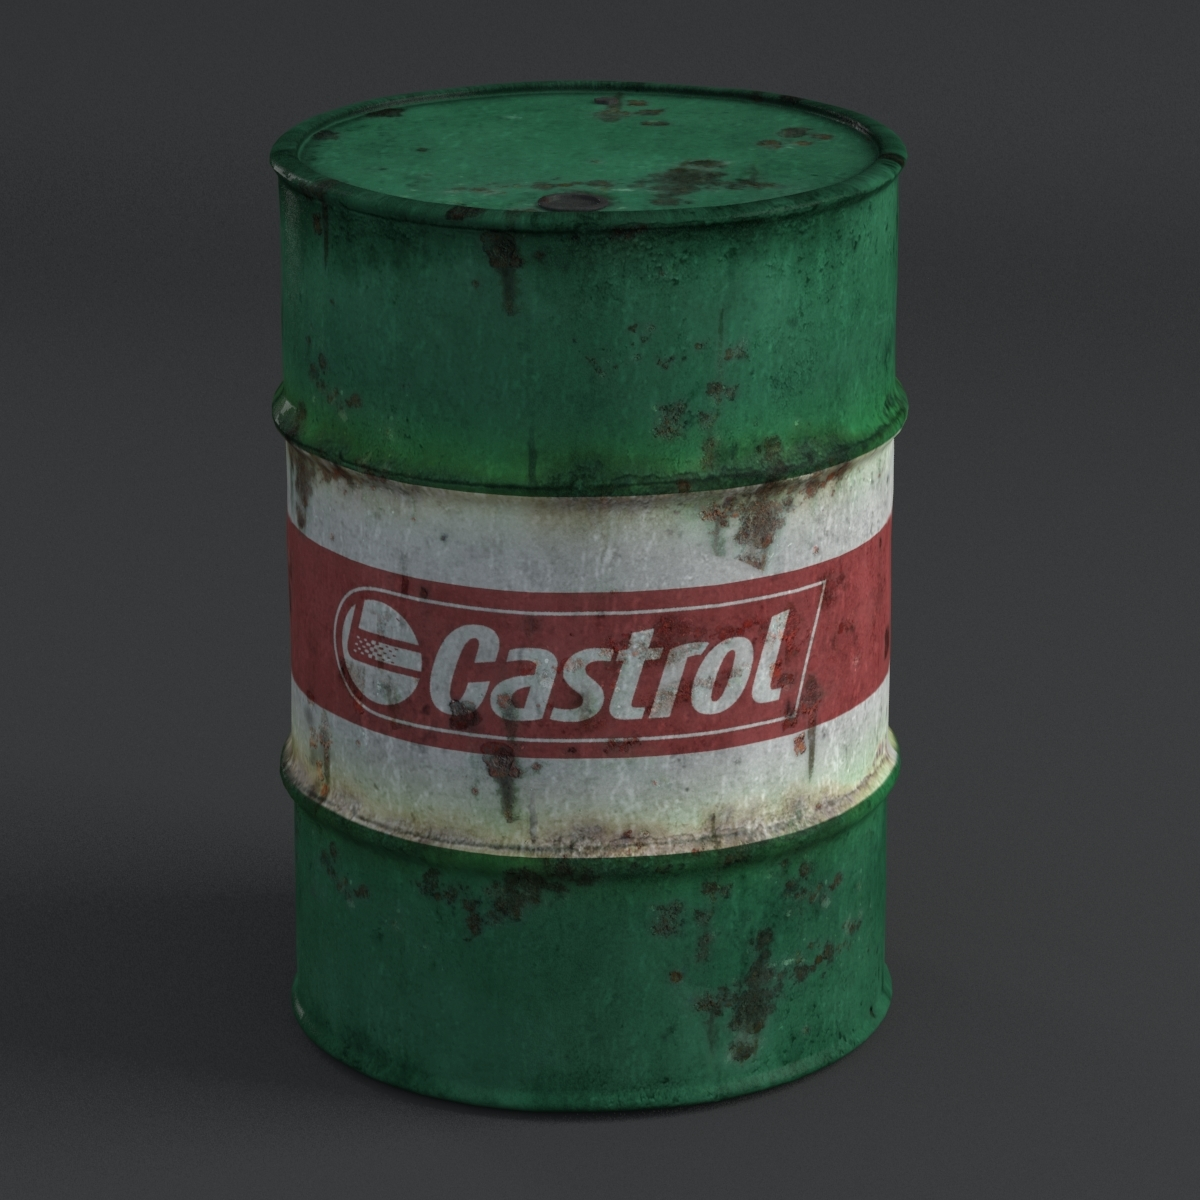
\includegraphics[width=1\linewidth]{barrelref.jpg}
  \caption{Zdjęcie poglądowe beczki Castrol.}\label{rys_2}
  \begin{minipage}[t]{0.75\linewidth}
    \emph{Źródło: indiamart.com | Castrol Oil Barrel}
  \end{minipage}
\end{figure}



\begin{figure}[!hbt]
\setcaptionwidth{1\linewidth}
\centering
  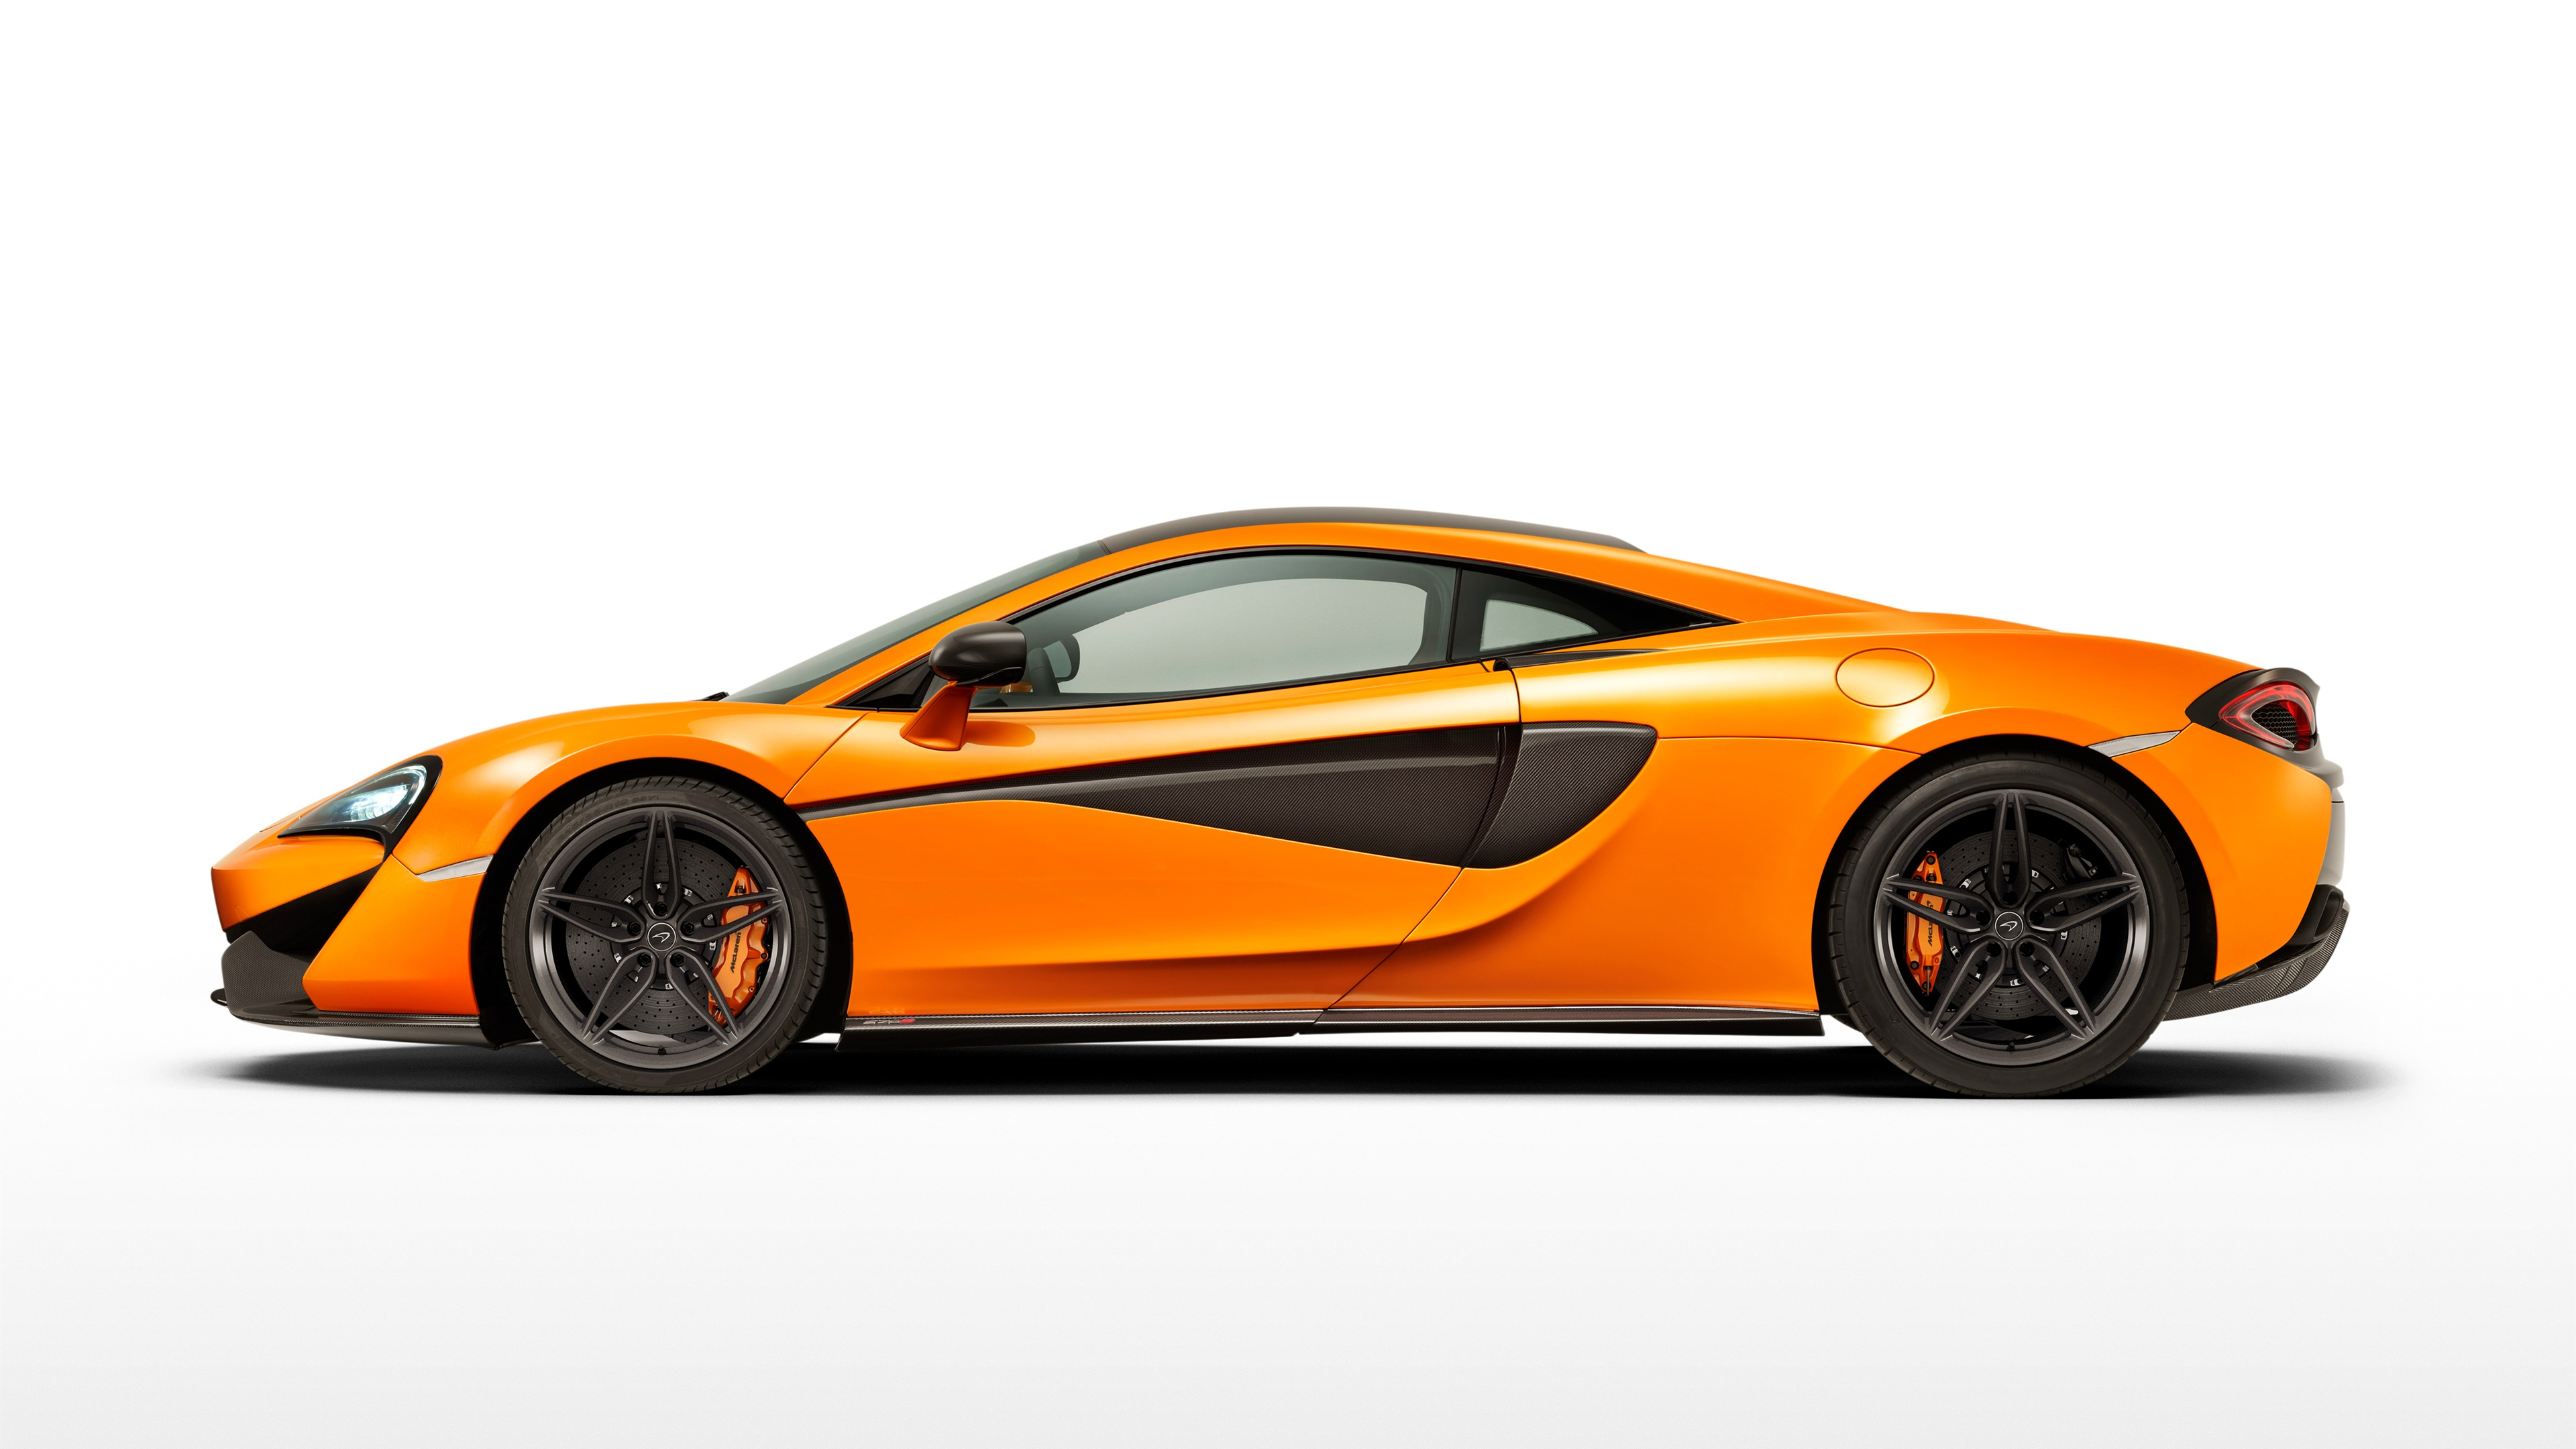
\includegraphics[width=1\linewidth]{carref.jpg}
  \caption{Zdjęcie poglądowe samochodu McLaren 570S.}\label{rys_3}
  \begin{minipage}[t]{0.75\linewidth}
    \emph{Źródło: kindpng.com | McLaren 570S side view}
  \end{minipage}
\end{figure}



\begin{figure}[!hbt]
\setcaptionwidth{1\linewidth}
\centering
  
\includegraphics[width=1\linewidth]{coneref.jpg}
  \caption{Zdjęcie poglądowe słupka drogowego.}\label{rys_4}
  \begin{minipage}[t]{0.75\linewidth}
    \emph{Źródło: flickr.com}
  \end{minipage}
\end{figure}




\newpage
\subsection{Modyfikatory obiektów}
\indent Istnieje wiele narzędzi w Blenderze, które pomagają uzyskać porządany przez nas efekt takie jak ,Mirror''. Uprzednio usuwając jedną połowę obiektu, dodając ten modyfikator na obiekt, otrzymuje się odbicie lustrzane ukazujące dwie identyczne połówki. Następnie modyfikując jedną stronę obiektu, ukazuje się identyczny wynik po drugiej stronie.

\begin{figure}[!hbt]
\setcaptionwidth{0.75\linewidth}
\centering
  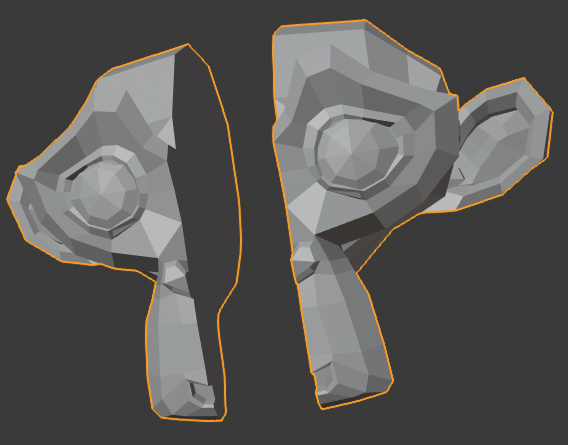
\includegraphics[width=1\linewidth]{mirror.png}
  \caption{Przykładowe zastosowanie modyfikatora Mirror.}\label{rys_5}
  \begin{minipage}[t]{0.75\linewidth}
    \emph{Źródło: Opracowanie własne}
  \end{minipage}
\end{figure}

\newpage

\indent Solidify służy do pogrubiania obiektów bez objętości. Płaskie elementy są pogrubiane dzięki czemu dalsze modyfikacje pozwalają uzyskać zupełnie inny wynik w przypadku płaskich obiektów.
\begin{figure}[!hbt]
\setcaptionwidth{1\linewidth}
\centering
  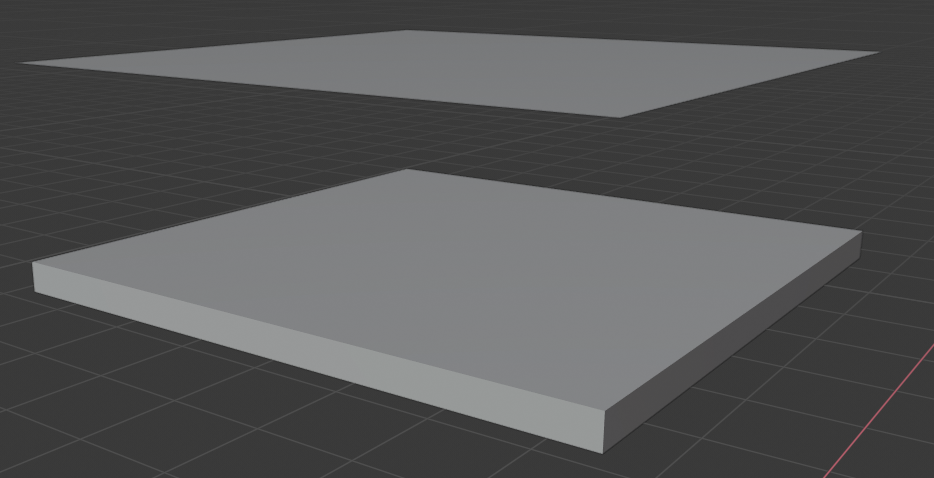
\includegraphics[width=0.7\linewidth]{solidify.png}
  \caption{Na górze kwadrat bez modyfikatora. Na dole z modyfikatorem Solidify.}\label{rys_6}
  \begin{minipage}[t]{0.75\linewidth}
    \emph{Źródło: Opracowanie własne}
  \end{minipage}
\end{figure}

\indent Bevel jest jednym z najlepszych narzędzi umieszczonych w Blenderze. Używając go, jesteśmy w stanie uzyskać efekt ściętych bądź zaokrąglonych krawędzi w zależności od podanej przez nas wartości.

\begin{figure}[!hbt]
\setcaptionwidth{0.75\linewidth}
\centering
  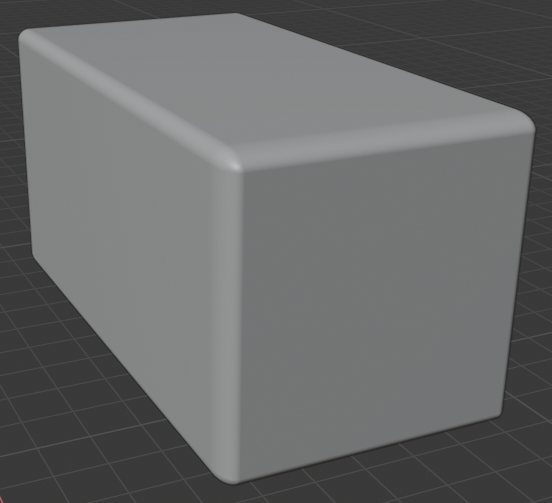
\includegraphics[width=0.7\linewidth]{bevel.png}
  \caption{Przykładowe zastosowanie modyfikatora Bevel.}\label{rys_7}
  \begin{minipage}[t]{0.75\linewidth}
    \emph{Źródło: Opracowanie własne}
  \end{minipage}
\end{figure}

\newpage
\indent ,,Decimate'' jest jednym z narzędzi pozwalających ograniczyć ilość punktów, czyli vertexów oraz ścian siatki meshowej, przy zachowaniu proporcji oraz kształtu obiektu. Podczas gdy obiekt zawiera kilka tysięcy poligonów, używa się tego modyfikatora aby zmiejszyć liczbę ścian, dzięki czemu uzyskuje się efekt low-poly. Możliwym jest zmiejszenie siatki meshowej o dany procent, ponieważ skala wartości zmian jest określona od 0 do 1 z dokładnością do czterech miejsc po przecinku. Ustawiając zmienną na 0.5 jesteśmy w stanie zmiejszyć liczbę poligonów o dokładnie 50\% \cite{3}.  Ponieważ pojazd jak i przeszkody zostały zbudowane od podstaw, nie było potrzeby zmniejszać ilości vertexów. W przypadku gdyby zostały użyte gotowe modele zawierające dużą ilość ścian, zostałby użyty modyfikator decimate.

\begin{figure}[!hbt]
\setcaptionwidth{1\linewidth}
\centering
  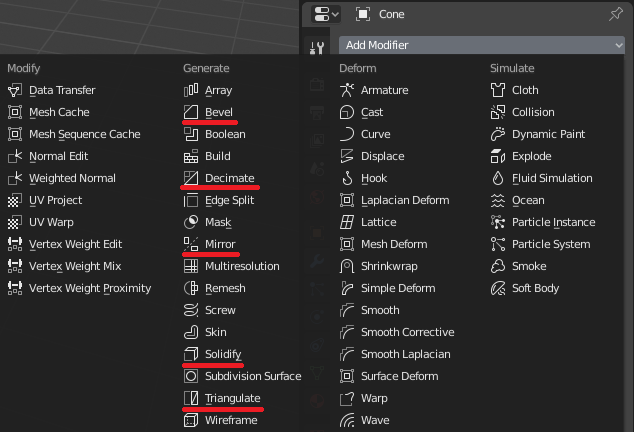
\includegraphics[width=1\linewidth]{modyfikatory.png}
  \caption{Zrzut ekrany z listą dostępnych modyfikatorów. Podkreślone zostały modyfikatory, które zostały użyte do stworzenia modeli pojazdu i przeszkód.}\label{rys_8}
  \begin{minipage}[t]{0.75\linewidth}
    \emph{Źródło: Opracowanie własne}
  \end{minipage}
\end{figure}

\subsection{Wireframe czyli siatka meshowa}
\indent Tworząc model który ma być wykonany w stylu low-poly, najważniejszym jest pierwsze spojrzenie. Obiekt o siatce złożonej tylko z poligonów wygląda gorzej niż obiekt składający się z trisów i poligonów. Jeżeli obiekt ma być animowany, dobrym pomysłem jest użycie modyfikatora ,,Triangulate''. Modyfikuje on siatkę meshową obiektu, przerabiając każdy poligon na dwa trisy zachowując przy tym geometrię obiektu. Podczas animowania obiektów, trisy zachowują się zdecydowanie lepiej od poligonów, które podczas np. przesuwania ręki, tworzą nienaturalne zagięcia. Ponieważ przeszkody jak i pojazd nie posiadają animacji obiekty dalej posiadają siatkę złożoną tylko z poligonów.

\begin{figure}[!hbt]
\setcaptionwidth{1\linewidth}
\centering
  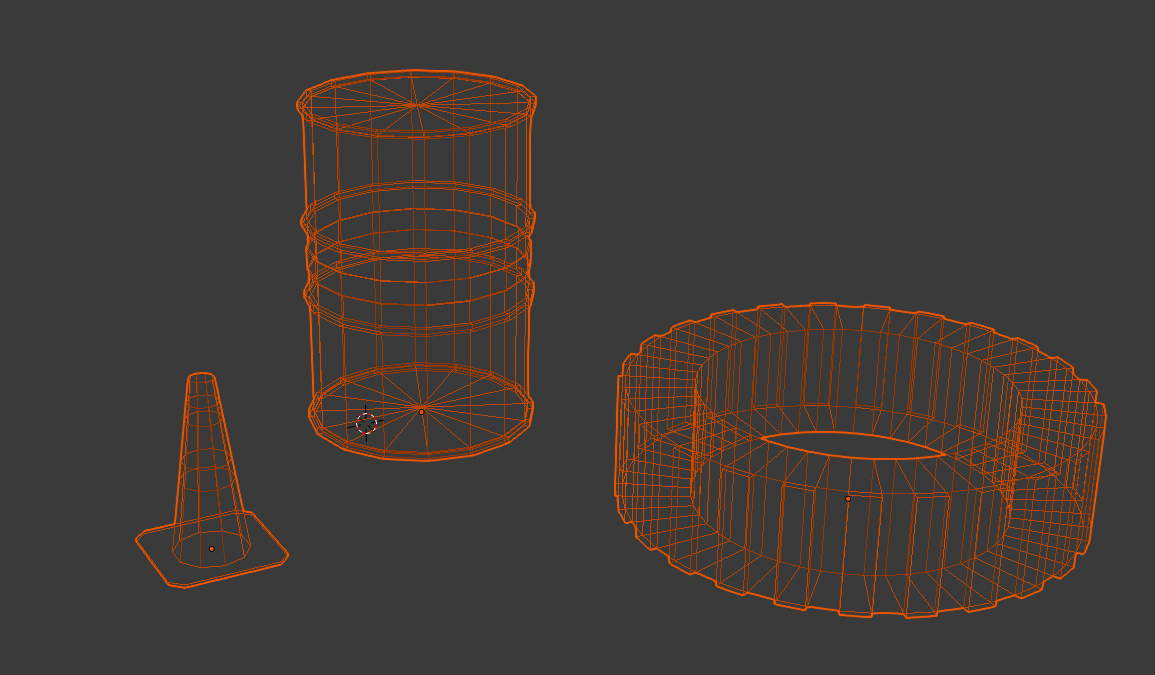
\includegraphics[width=1\linewidth]{wireframe.png}
  \caption{Siatka meshowa przeszkód.}\label{rys_9}
  \begin{minipage}[t]{0.75\linewidth}
    \emph{Źródło: Opracowanie własne}
  \end{minipage}
\end{figure}

\newpage
\subsection{Tworzenie modelu 3D pojazdu}
\indent Tworząc obiekt zazwyczaj zaczyna się od zwykłej kostki sześciennej, którą następnie modyfikuje się poprzez przesuwanie vertexów, krawędzi bądź całych ścian obiektu. Blender posiada niesamowitą umiejętność łączenia funkcji. Przykładowo, korzystając ze skrótów klawiszowych, twórca jest w stanie wysuwać ścianę obiektu a następnie ją skalować nie przerywając wysuwania. \textbf{Pojazd} został stworzony korzystając ze zdjęcia poglądowego McLaren'a 570S ustawionego w widoku side view (bocznym) oraz własnej wyobraźni, aby uzyskać kształt przypominający bryłę tego samochodu. Za pomocą narzędzia Extrude dodano dodatkowe ściany, dzięki którym możliwym jest uzyskanie kształtu potrzebnej do odwzorowania modelu rzeczywistego. Jest to jedno z najważniejszych narzędzi, dzięki któremu jesteśmy w stanie uzyskać geometrię, która pozwoli stworzyć dokładniejszy obiekt, który będzie posiadał dodatkowe detale. Następnie można było ustawiać krawędzie obiektu nadając mu kształt przypominający ten na zdjęciu.

\begin{figure}[!hbt]
\setcaptionwidth{1\linewidth}
\centering
  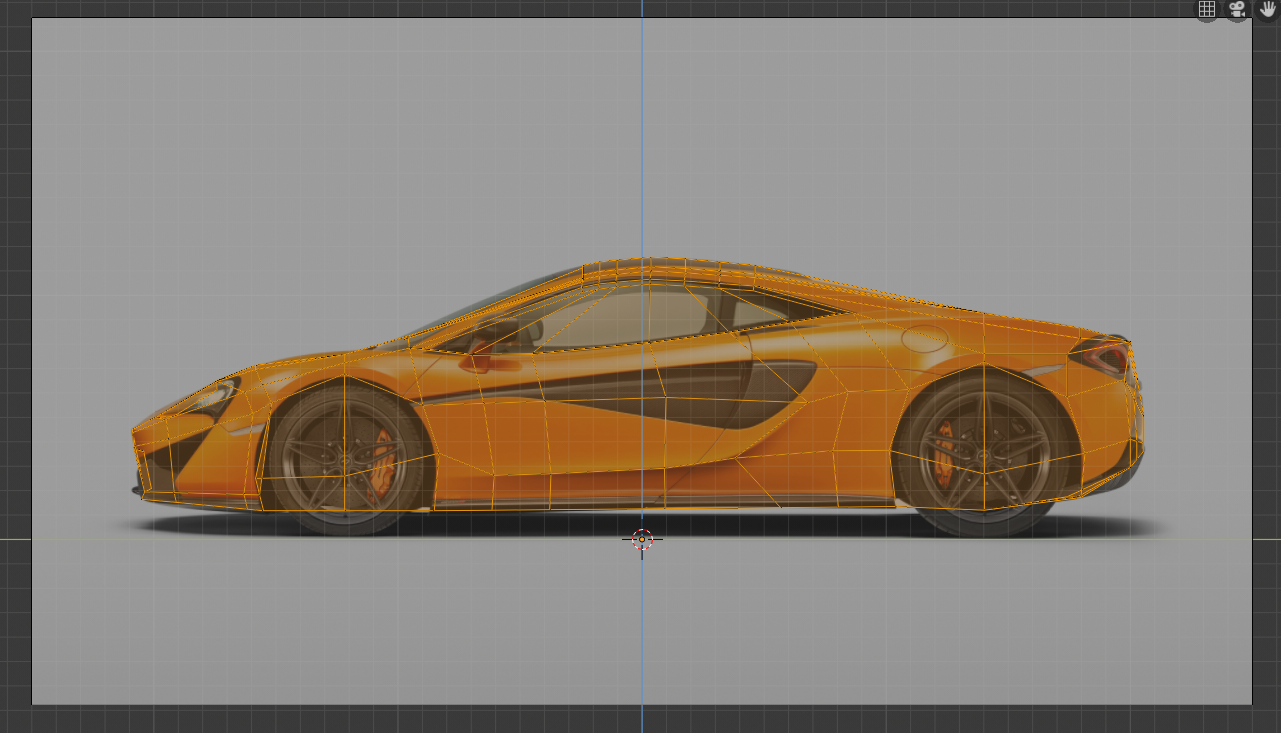
\includegraphics[width=1\linewidth]{ksztalt.png}
  \caption{Siatka modelu w widoku Wireframe pokazująca ułożenie krawędzi pojazdu na zdjęciu referencyjnym.}\label{rys_10}
  \begin{minipage}[t]{0.75\linewidth}
    \emph{Źródło: Opracowanie własne}
  \end{minipage}
\end{figure}

%%%%%%
\newpage
\indent Ustawiając wszystkie krawędzie, aby pasowały do zdjęcia referencyjnego, umiejscowiono krawędzie siatki w taki sposób, aby możliwym było wysunięcie wszystkich ścian bocznych poza miejscem na koła. W ten sposób za pomocą narzędzia Extrude, uzyskano nadkola pojazdu. Następnym krokiem, było stworzenie koła. W środku nadkola, dodano Circle, czyli okrąg. Bazowo okrąg posiada 32 ściany, lecz zmiejszono ich liczbę do 16 za pomocą narzędzia dodawania okręgu. Następnie dopasowano go do rozmiaru opony, za pomocą narzędzia skalowania. Również przy pomocy narzędzia Extrude, stworzono walec bez ścian zamykających go. Przy pomocy Extrude, którego przesunięcie zostało anulowane poprzez prawy przycisk myszy, stworzono dwie linie, które są umieszczone na płaszczyźnie koła, które następnie zostały zeskalowane do centralnej linii opony, a następnie przy pomocy Extrude zmniejszono do rozmiarów środka koła i wysunięto na zewnątrz koła, aby uzyskać efekt prawdziwej felgi. 

\begin{figure}[!hbt]
\setcaptionwidth{1\linewidth}
\centering
  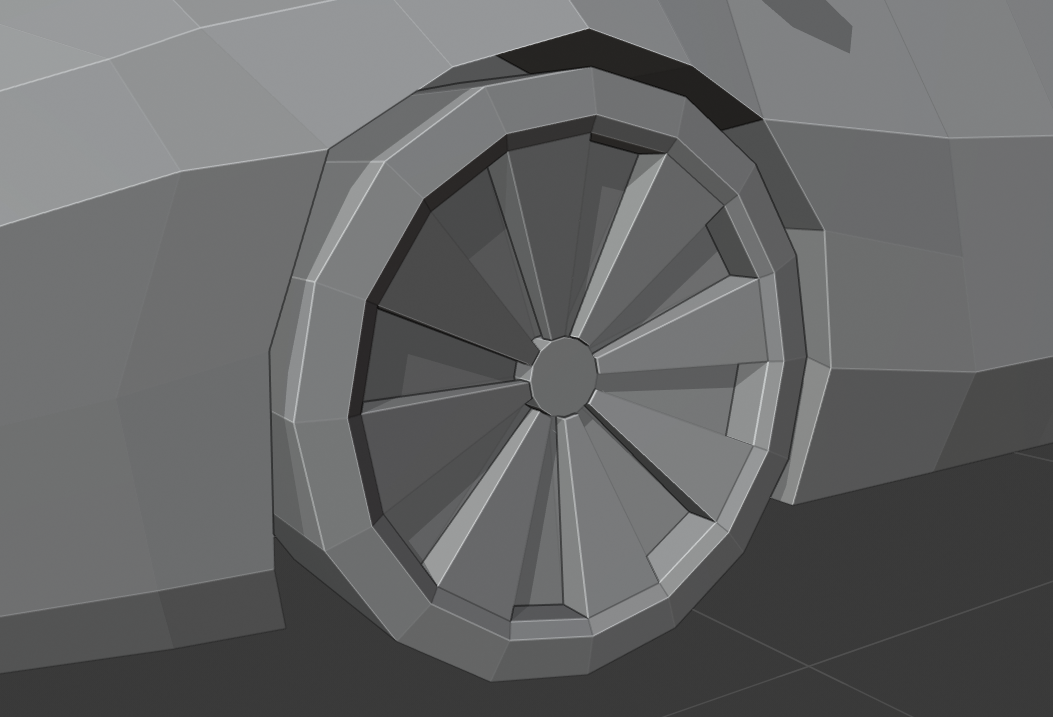
\includegraphics[width=0.7\linewidth]{opona.png}
  \caption{Ilustracja przedstawiająca koło pojazdu.}\label{rys_11}
  \begin{minipage}[t]{0.75\linewidth}
    \emph{Źródło: Opracowanie własne}
  \end{minipage}
\end{figure}

Wybierając co drugą ścianę felgi, uzyskano 8 elementów, które za pomocą Extrude, którego przesunięcie zostało anulowane oraz narzędzia skalowania dopasowano do środka felgi, aby imitowały połączenie z wystającym walcem. Aby uzyskać efekt takiego samego koła użyto modyfikatora Mirror, aby odbił obiekt na płaszczyźnie Y. Następnie koło z modyfikatorem Mirror, który nie jest jeszcze zaakceptowany, zduplikowano aby dodać koła na tylną część pojazdu.

\indent W każdym pojeździe muszą być lusterka boczne. Aby stworzyć lusterko, wykorzystano plane, czyli płaski kwadrat, który następnie umieszczono pod karoserią drzwi i użyto narzędzia Extrude. Dzięki możliwości przesuwania vertexów oraz skalowania, twórca jest w stanie uzyskać kształt lusterka, który w głównej mierze przypomina prawdzwe lusterko sportowego samochodu.

\begin{figure}[!hbt]
\setcaptionwidth{1\linewidth}
\centering
  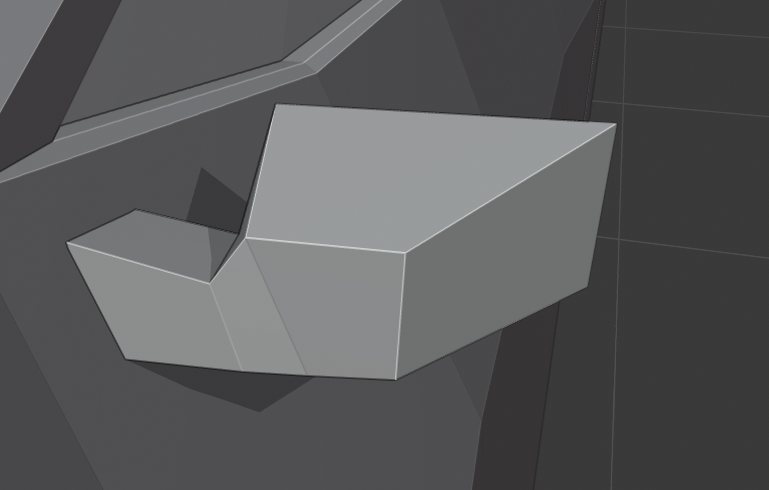
\includegraphics[width=0.8\linewidth]{lusterko.png}
  \caption{Ilustracja przedstawiająca lusterko boczne umieszczone na drzwiach pojazdu.}\label{rys_12}
  \begin{minipage}[t]{0.75\linewidth}
    \emph{Źródło: Opracowanie własne}
  \end{minipage}
\end{figure}

\indent Aby obiekt posiadał kolory, wykorzystano zawartą w Blenderze opcję materiałów. Na dany obiekt, można dodać nieskończenie wielką liczbę materiałów. Każdy z nich może posiadać różne właściwości, takie jak szorstkość, reflektywność odbić czy też emisja koloru. Zdecydowano, że pojazd będzie posiadał jasny odcień koloru niebieskiego z maksymalną szorstkością oraz wyglądem metalicznym zwiększonym do 0.5. Aby dodać materiał na obiekt, należy wybrać wszystkie vertexy, które tworzą ściany, a następnie zatwierdzić je poprzez przycisk Assign. Przypisuje on danym elementom modelu jeden materiał. \\ Ponieważ Koła są również połączone z modelem samochodu, automatycznie dostały ten sam kolor. Koniecznym jest powtórzenie poprzedniego kroku, aby dodać inny materiał na opony oraz felgi. 
%%%%%%

\begin{figure}[!hbt]
\setcaptionwidth{1\linewidth}
\centering
  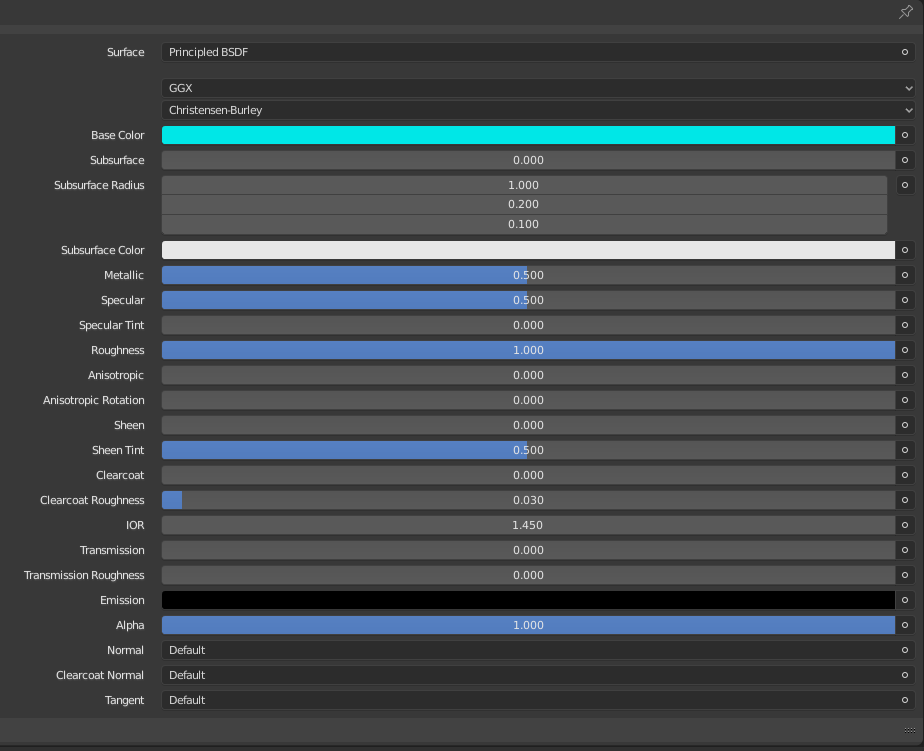
\includegraphics[width=0.8\linewidth]{materialcar.png}
  \caption{Okno modyfikacji materiału nałożonego na siatkę pojazdu.}\label{rys_13}
  \begin{minipage}[t]{0.75\linewidth}
    \emph{Źródło: Opracowanie własne}
  \end{minipage}
\end{figure}

\begin{figure}[!hbt]
\setcaptionwidth{1\linewidth}
\centering
  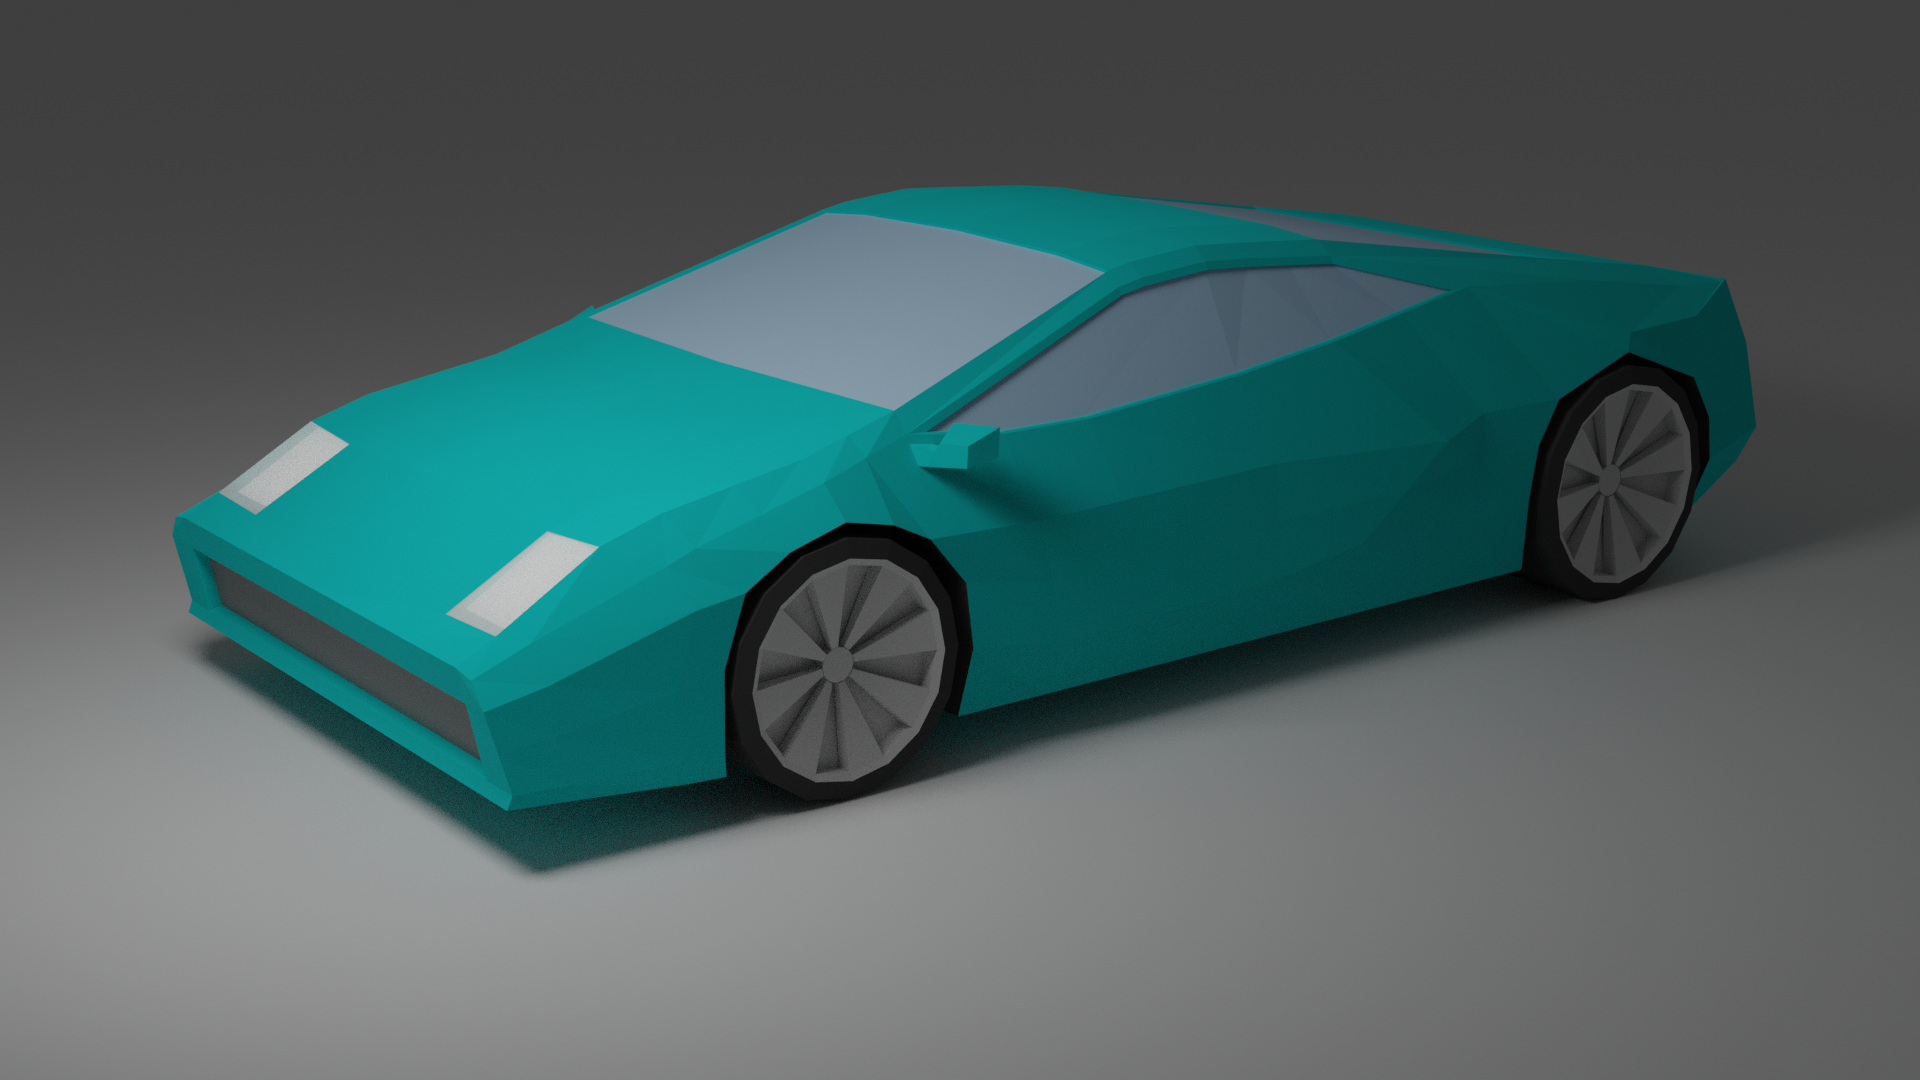
\includegraphics[width=0.8\linewidth]{car.png}
  \caption{Render gotowego pojazdu stworzonego na potrzeby projektu.}\label{rys_14}
  \begin{minipage}[t]{0.75\linewidth}
    \emph{Źródło: Opracowanie własne}
  \end{minipage}
\end{figure}

%%%%%%
\newpage
\subsection{Tworzenie modelu 3D przeszkód}
\indent Aby stworzyć \textbf{słupek drogowy}, wykorzystano cylinder, którego liczbę ścian ustawiono na 10. Następnie zmniejszono rozmiar górnej płaszczyzny za pomocą narzędzia skalowania, dzięki czemu możliwym było uzyskanie stożkowego wyglądu. Dodając do sceny plane, czyli płaski kwadrat, została stworzona podstawa słupka. Aby uzyskać efekt ściętych rogów kwadratu, użyto modyfikatora Bevel, który zaokrągla krawędzie. W przypadku płaskiego kwadratu, modyfikator ten nie daje żadnego efektu. Modyfikator Bevel posiada opcję, która pozwala ściąć rogi, czyli z jednego vertexa tworzy dwa i odpowiednio więcej w przypadku zwiększenia ilości cięć. Następnie użyto modyfikatora Solidify, który powoduje pogrubienie płaszczyzny nadając jej potrzebnej geometrii i objętości. Aby wyeksportować modele jako plik .fbx należy zaakceptować obydwie modyfikacje w odpowiedniej kolejności, od góry do dołu. Aby połączyć cylinder z kwadratem użyto skrótu klawiszowego Ctrl + J, który łączy zaznaczone obiekty w jeden.

\indent Tworząc \textbf{beczkę} oraz \textbf{oponę}, wykorzystano identyczne narzędzia jak w przypadku słupka drogowego. Różnicą był ilość ścian obiektu oraz sposób w jaki były przesuwane krawędzie boczne modelu.

\begin{figure}[!hbt]
\setcaptionwidth{0.75\linewidth}
\centering
  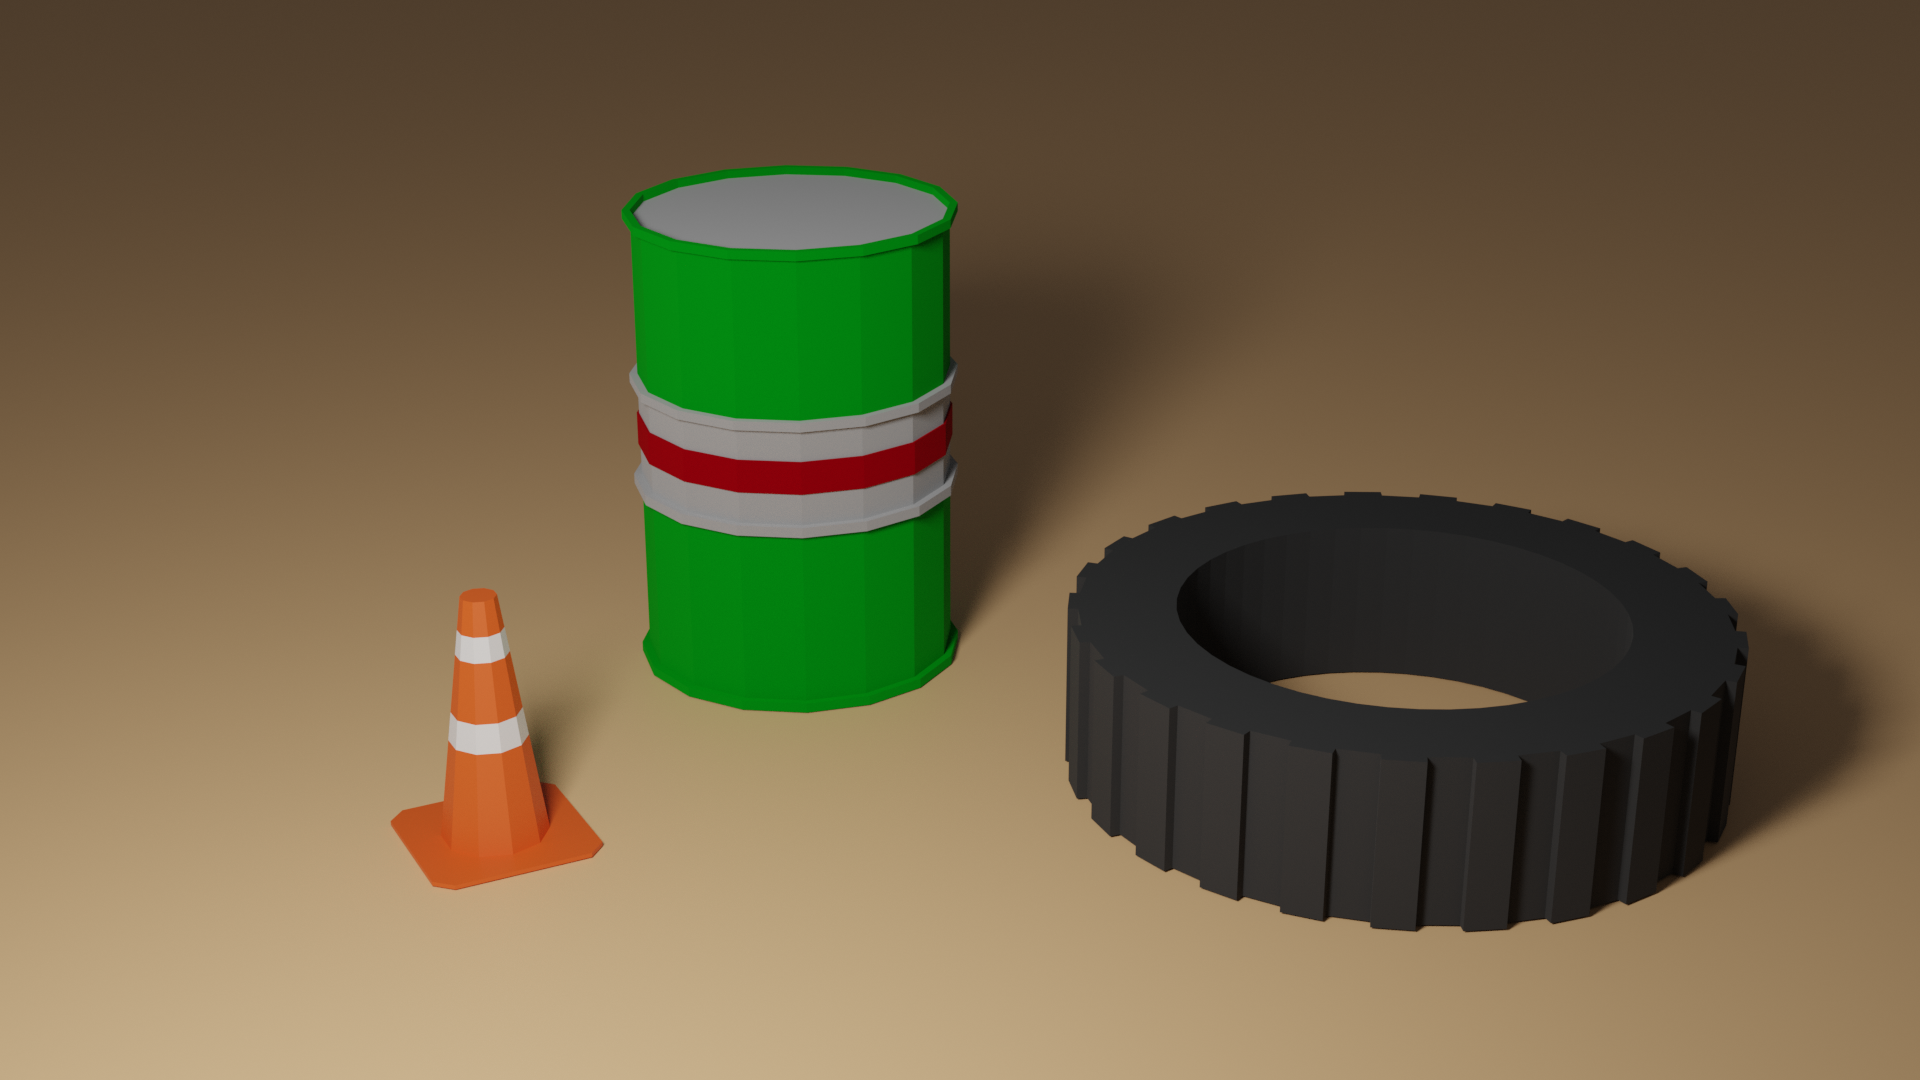
\includegraphics[width=0.8\linewidth]{przeszkody.png}
  \caption{Przeszkody stworzone w Blenderze.}\label{rys_15}
  \begin{minipage}[t]{0.75\linewidth}
    \emph{Źródło: Opracowanie własne}
  \end{minipage}
\end{figure}


\newpage
\section{Środowisko Unity}
%%%%%%
\indent Obiekty stworzone w Blenderze, zostały wyeksportowane jako plik typu fbx, który idealnie przechowuje dane obiektu, takie jak siatka meshowa, materiały nałożone na obiekt, oraz animacje. Niestety skala obiektów nie jest zachowana, a modele posiadają skalę 100 jednostek Unity. Aby przeszkody nie wisiały w powietrzu, została stworzona płaska powierzchnia o rozmiarach 15x3x1000 jednostek Unity. Następnie umieszczono wszystkie obiekty w scenie. Korzystając z zawartych w programie komponentów nadano każdemu modelowi komponent Mesh Collider, który odpowiada za wykrywanie kolizji z innymi obiektami, oraz Rigidbody będący głównym elementem fizyki obiektów. Aby obiekty posiadały rozsądne rozmiary, zostały zmodyfikowane ich gabaryty. Następnie zmodyfikowano ich masy w komponencie RigidBody tak, aby pojazd się od nich odbijał. Po dokonaniu zmian zostały stworzone prefaby. Prefabem nazywany jest ten sam obiekt, który po ponownym umieszczeniu w scenie posiada te same właściwości. Dodatkowo gotowe prefaby można używać w późniejszych etapach, przykładowo losowo generowany poziom, który w wyznaczonych miejscach ustawia losowy obiekt. Na potrzeby tego projektu stworzono gotowe poziomy, ze względu na aktualny stan oraz komplikacje związane z rozmiarem projektu. Ustawiając obiekty na powierzchni, stworzono 5 różnych poziomów, które różnią się trudnością, odpowiednio od pierwszego do piątego. Każdy z nich jest bardziej skomplikowany. 


\newpage
\subsection{Scenariusz rozgrywki}
\indent Po uruchomieniu gry, ukazuje się menu główne na którym znajduje się nazwa gry, przycisk do włączenia gry, oraz do wyjścia z programu. Głównym zadaniem gracza jest przejechanie samochodem przez pięć poziomów bez dotknięcia żadnej przeszkody. W przypadku kiedy pojazd udeży przeszkodę, poziom na którym polegliśmy jest ładowany od nowa z opóźnieniem dwu sekundowym, aby gracz mógł zobaczyć kolizję pojazdu z przeszkodą. Jeżeli graczowi uda się przejść wszystkie pięć poziomów ukazuje mu się ekran końcowy na którym widnieją gratulacje oraz przycisk do wyłączenia programu.

\begin{figure}[!hbt]
\setcaptionwidth{1\linewidth}
\centering
  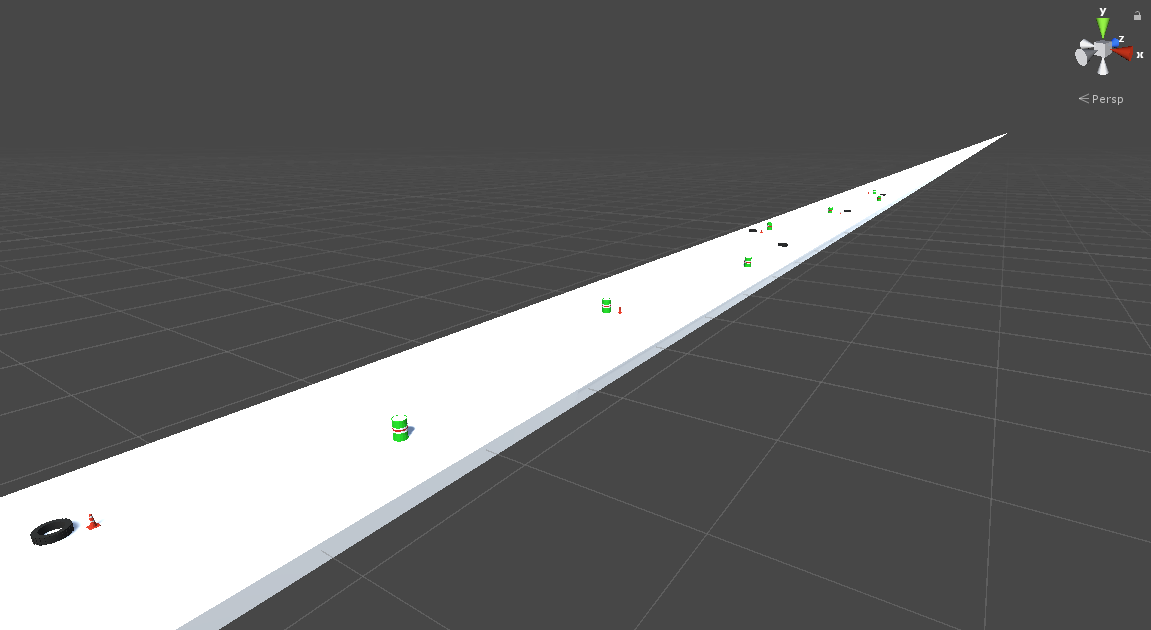
\includegraphics[width=1\linewidth]{scena1.png}
  \caption{Ustawienie przeszkód na poziomie 1.}\label{rys_16}
  \begin{minipage}[t]{0.75\linewidth}
    \emph{Źródło: Opracowanie własne}
  \end{minipage}
\end{figure}

\newpage
\begin{figure}[!hbt]
\setcaptionwidth{1\linewidth}
\centering
  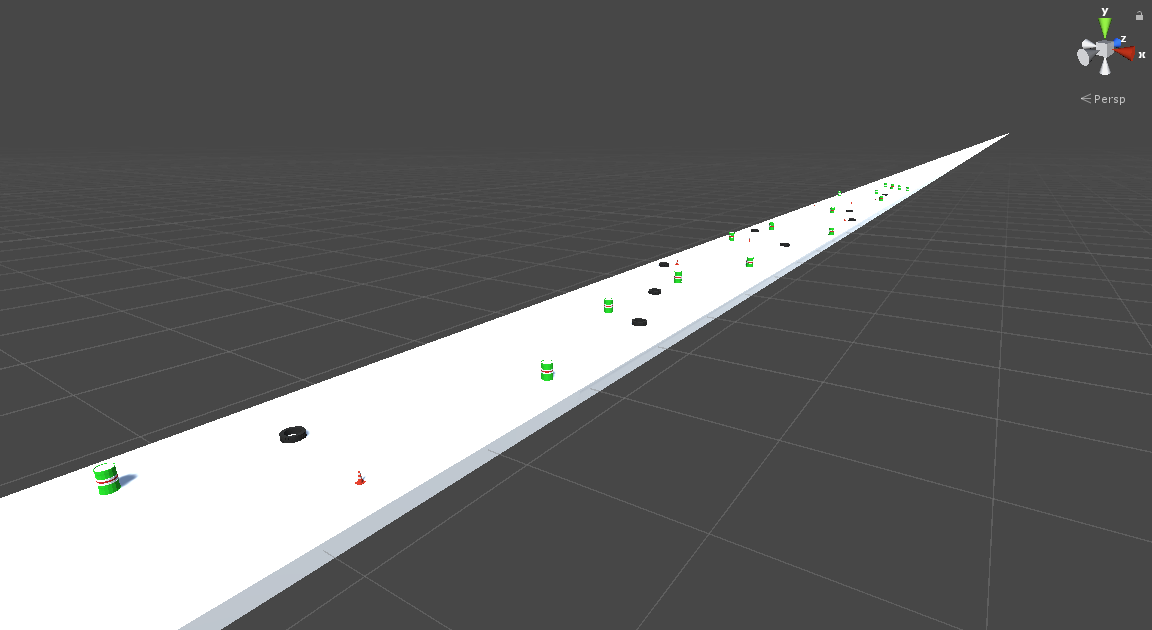
\includegraphics[width=1\linewidth]{scena3.png}
  \caption{Ustawienie przeszkód na poziomie 3.}\label{rys_17}
  \begin{minipage}[t]{0.75\linewidth}
    \emph{Źródło: Opracowanie własne}
  \end{minipage}
\end{figure}

\begin{figure}[!hbt]
\setcaptionwidth{1\linewidth}
\centering
  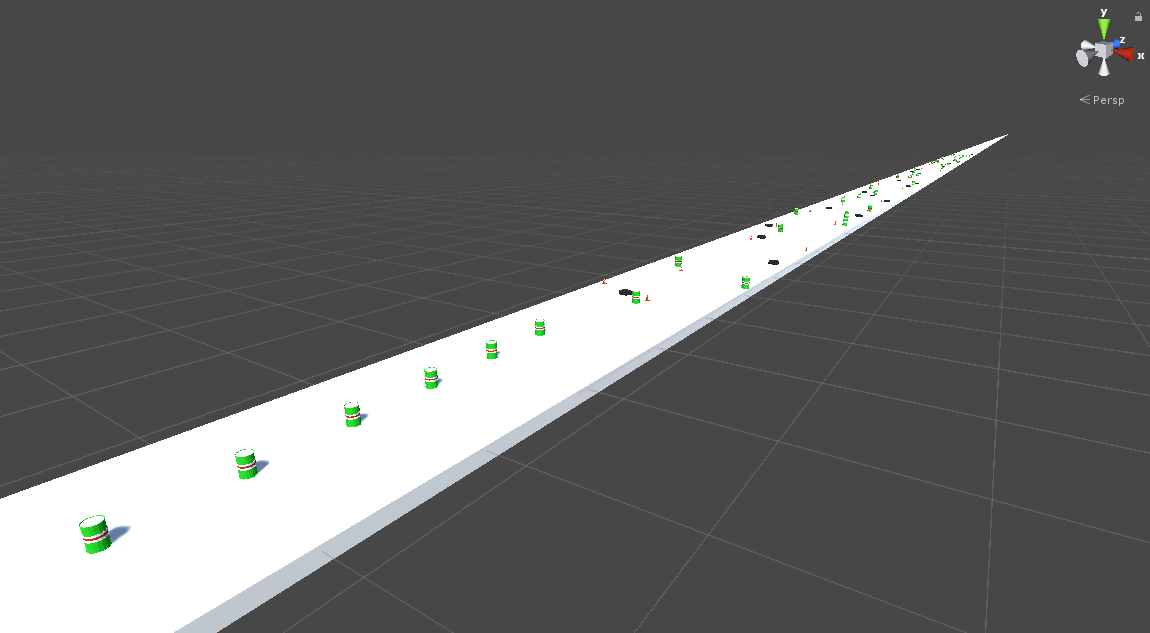
\includegraphics[width=1\linewidth]{scena5.png}
  \caption{Ustawienie przeszkód na poziomie 5.}\label{rys_18}
  \begin{minipage}[t]{0.75\linewidth}
    \emph{Źródło: Opracowanie własne}
  \end{minipage}
\end{figure}

\newpage
\subsection{Materiał poślizgowy}
\indent Pojazd podczas poruszania się wykrywa tarcie pomiędzy sobą a powierzchnią planszy. Aby uniknąć niechcianych podskoków pojazdu, stworzono w Unity materiał specjalny, który wpływa na fizykę komponentów RigidBody umieszczonych na pojeździe oraz przeszkodach. Zmienne Dynamic Friction oraz Static Friction zmieniono na 0, a następnie dodano material SlipperMat na planszę gry.


\begin{figure}[!hbt]
\setcaptionwidth{1\linewidth}
\centering
  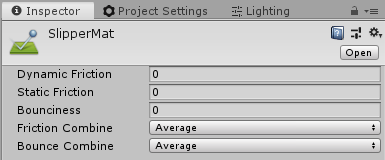
\includegraphics[width=1\linewidth]{slippermat.png}
  \caption{Materiał SlipperMat, który został dodany na powierzchnię planszy}\label{rys_19}
  \begin{minipage}[t]{0.75\linewidth}
    \emph{Źródło: Opracowanie własne}
  \end{minipage}
\end{figure}
%%%%%%
\newpage
\subsection{Animacje}
\indent Przejścia pomiędzy poziomami będą zawierały krótką i prostą animację wyświetlającą wiadomość ,,LEVEL COMPLETE''. Tworzenie animacji polega na stworzeniu Panelu z tekstem a następnie na osi czasu zmiany wartości alfy, tak aby napis oraz tło pojawiły się. W sekcji programowania znajduje się kod odpowiedzialny za proces przejścia z jednego poziomu na drugi.


\begin{figure}[!hbt]
\setcaptionwidth{1\linewidth}
\centering
  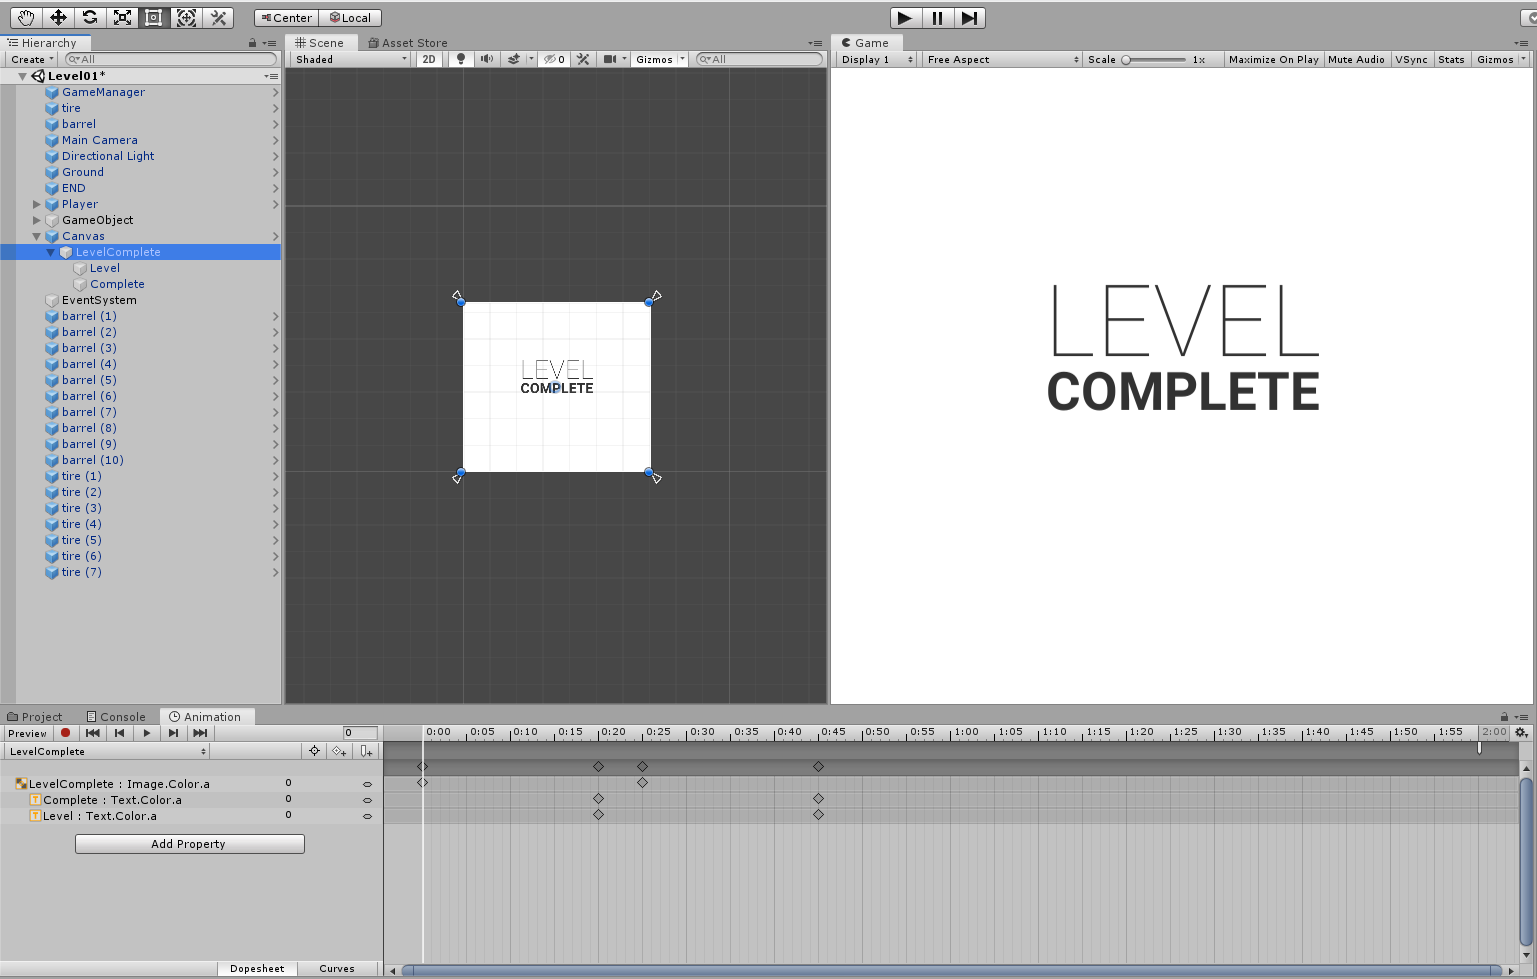
\includegraphics[width=1\linewidth]{levelcomplete2.png}
  \caption{Zrzut ekranu pokazujący oś czasu oraz wynik animacji.}\label{rys_20}
  \begin{minipage}[t]{0.75\linewidth}
    \emph{Źródło: Opracowanie własne}
  \end{minipage}
\end{figure}


\newpage
\section{Programowanie skryptów}
%%%%%%
\subsection{Poruszanie pojazdem}
\indent Programowanie zaczęto od stworzenia skryptu obsługującego poruszanie się pojazdem. Aby obiekt się poruszał, wykorzystano komponent Rigidbody umieszczony na samochodzie. Korzystając z gotowych funkcji zawartch w Rigidbody, mianowicie \textit{AddForce()}, można sprawić aby obiekt poruszał się w danym kierunku z określoną mocą. 

\begin{figure}[!h]
\setcaptionwidth{0.75\linewidth}
\centering
  \includegraphics[width=1\linewidth]{playermove.png}
  \caption{Skrypt PlayerMovement obsługujący poruszanie się pojazdu po poziomie.}\label{rys_21}
  \begin{minipage}[t]{0.75\linewidth}
    \emph{Źródło: Opracowanie własne}
  \end{minipage}
\end{figure}

\newpage
\indent Ponieważ nie każdy komputer posiada taką samą prędkość liczenia klatek, do zmiennej określającej prędkość pojazdu dodano \textit{Time.deltaTime}. Wartość ta, określa czas pomiędzy klatkami, które uzyskuje komputer. Dzięki takiemu rozwiązaniu, rozgrywka będzie wyglądać tak samo na komputerze z tego roku jak i na komputera z przed dekady. \cite{4} Ponieważ na pojazd, został nałożony komponent RigidBody, obiekt posiada swoją masę. RigidBody jako komponent określający fizykę, oblicza zachowanie każdego obiektu w sposób przypominający w dużym stopniu prawdziwe prawa fizyki. Na każdy obiekt działa siła przyciągania ziemskiego zwiększona o masę. Takie rozwiązanie wpływa negatywnie na pojazd podczas ruchu w przód oraz skręcania. Zdecydowano dodać czwartą zmienną. \textit{ForceMode.VelocityChange} dodaje natychmiastową zmianę prędkości ciału, pomijając z obliczeń jego masę. Rozwiązanie to przydaje się w przypadku, kiedy na scenie znajduje się wiele obiektów, które poruszają się z tą samą prędkością, ale posiadają inne rozmiary i masy. Okazałoby się, że przykładowy rower, który jedzie z prędkością np. 50 km/h będzie jechał szybciej od dużej ciężarówki, która również porusza się z taką samą prędkością. \cite{5}

\indent FindObjectOfType służy do przeszukuwania katalogów gry pod względem tego co zostało napisane w nawiasach ostrokątnych. Ponieważ w skrypcie GameManager została napisana funkcja \textit{EndGame()} FindObjectOfType szuka GameManagera, aby następnie uzyskać dostęp do funkcji, która musi być ustawiona na public, inaczej nie zostanie uruchomiona, a Unity pokaże błąd.

\begin{figure}[!h]
\setcaptionwidth{0.75\linewidth}
\centering
  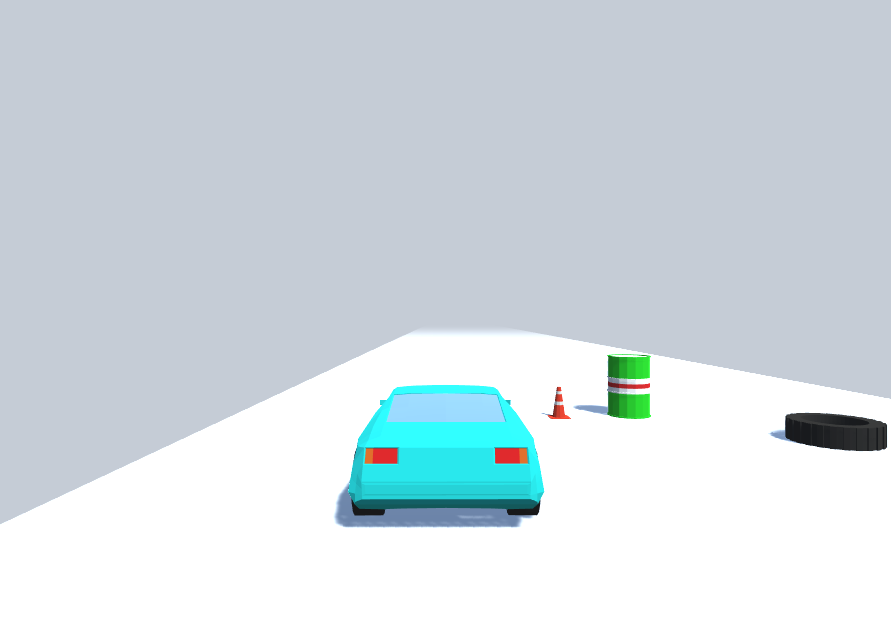
\includegraphics[width=1\linewidth]{carmove.png}
  \caption{Zdjęcie ukazujące pojazd, który zboczył z trasy, efekt skryptu ruchu.}\label{rys_22}
  \begin{minipage}[t]{0.75\linewidth}
    \emph{Źródło: Opracowanie własne}
  \end{minipage}
\end{figure}

\indent Kamera musi śledzić gracza, dlatego napisano skrypt, który ustala pozycję kamery w świecie gry, na taką samą pozycję co pojazd, jednakże dodany jest offset czyli przesunięcie, które podnosi kamerę do góry i przesuwa ją do tyłu, tak aby widok był z perspektywy trzeciej osoby.

\begin{figure}[!h]
\setcaptionwidth{0.75\linewidth}
\centering
  \includegraphics[width=1\linewidth]{followplayer.png}
  \caption{Skrypt FollowPlayer obsługujący umieszczenie kamery za pojazdem.}\label{rys_23}
  \begin{minipage}[t]{0.75\linewidth}
    \emph{Źródło: Opracowanie własne}
  \end{minipage}
\end{figure}
\newpage
\subsection{Obsługa kolizji}
\indent Kolejnym zadaniem było napisanie skryptu, który będzie wykrywał kolizje z przeszkodami oraz resetował poziom, jeżeli pojazd spadnie z planszy. Ponieważ platforma po której porusza się pojazd, również jest wykrywana jako kolizja, wszystkie przeszkody zostały otagowane jako ,,Obstacle''. W skrypcie PlayerMovement został dodany kod obsługujący resetowanie poziomu, jeżeli wartość y pojazdu spadnie poniżej -1, który odwołuje się do funkcji \textit{EndGame()} w skrypcie GameManager.

\begin{figure}[!hbt]
\setcaptionwidth{0.75\linewidth}
\centering
  \includegraphics[width=1\linewidth]{playercollision.png}
  \caption{Skrypt PlayerCollision obsługujący kolizje pomiędzy pojazdem a przeszkodami.}\label{rys_24}
  \begin{minipage}[t]{0.75\linewidth}
    \emph{Źródło: Opracowanie własne}
  \end{minipage}
\end{figure}

\newpage
\begin{figure}[!hbt]
\setcaptionwidth{0.75\linewidth}
\centering
  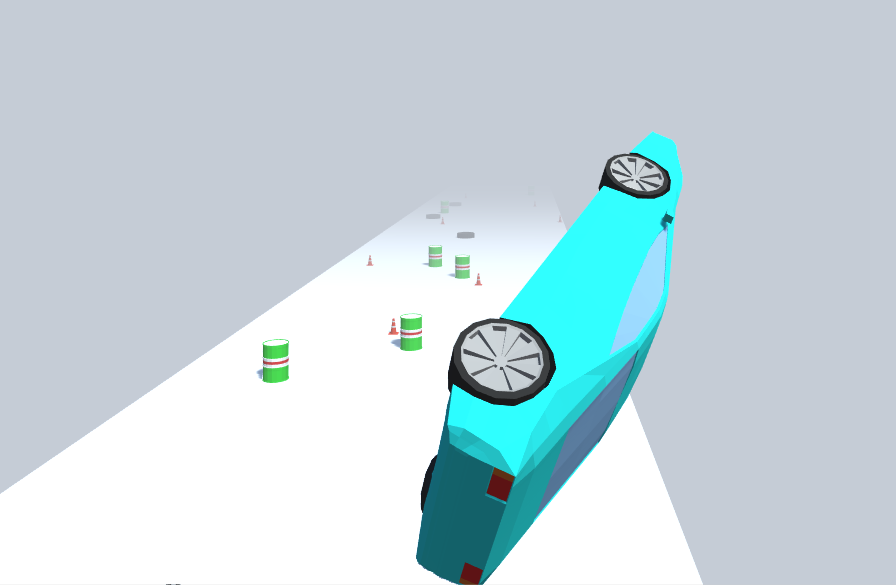
\includegraphics[width=1\linewidth]{kolizja1.png}
  \caption{Przykładowa kolizja, która wyrzuciła pojazd do góry.}\label{rys_25}
  \begin{minipage}[t]{0.75\linewidth}
    \emph{Źródło: Opracowanie własne}
  \end{minipage}
\end{figure}

\indent Ponieważ w inspektorze nie da się podpiąć skryptu GameManager do prefabu pojazdu, w skrypcie PlayerCollision znajduje się metoda \textit{FindObjectOfType} która przeszukuje w lokalizacji skryptów plik o nazwie GameManager a następnie korzysta z jego funkcji która musi być ustawiona jako publiczna. Stworzono typ logiczny bool gameHasEnded, który przybiera dwie wartości, prawda lub fałsz, którego wartość zmieniana jest przy pierwszym uruchomieniu funkcji, aby upewnić się, że funkcja będzie ładowana tylko jeden raz. Następnie po upadku, bądź kolizji, poziom jest ładowany od nowa, tak więc gameHasEnded ma swoją pierwotną wartość. 

\newpage
\indent Aby gra nie resetowała się za szybko, zamiast uruchamiać funkcję \textit{EndGame()} od razu, wykorzystano metodę \textit{Invoke} która po dodaniu nazwy funkcji, oraz czasu w sekundach, uruchamia funkcję w określonym przez twórce czasie. Aby przejść na następny poziom, gracz musi przejechać pomiędzy przeszkodami tak żeby ich nie dotknąć. W przypadku porażki poziom zostanie załadowany od nowa.

\begin{figure}[!hbt]
\setcaptionwidth{0.75\linewidth}
\centering
  \includegraphics[width=1\linewidth]{gamemanager.png}
  \caption{Skrypt GameManager zajmujący się restowaniem poziomów.}\label{rys_26}
  \begin{minipage}[t]{0.75\linewidth}
    \emph{Źródło: Opracowanie własne}
  \end{minipage}
\end{figure}
%%%%%%

\newpage
\subsection{Ładowanie poziomów}
\indent Poziom jest już możliwy do przejścia, jednakże trzeba załadować kolejny. Na końcu trasy każdego z poziomów umieszczono kostkę o szerokości 15 jednostek Unity, która jest niewidoczna i służy jako przełącznik uruchamiający animację zakończonego poziomu, oraz ładuje kolejny. W skrypcie EndTrigger znajduje się jedna funkcja \textit{OnTriggerEnter()}, która ładuje funkcję \textit{CompleteLevel()} ze skryptu GameManager odpowiedzialną za włączenie animacji zakończenia poziomu.

\begin{figure}[!ht]
\setcaptionwidth{0.75\linewidth}
\centering
  \includegraphics[width=0.8\linewidth]{endtrigger.png}
  \caption{Skrypt EndTrigger nawiązujący do GameManager.}\label{rys_27}
  \begin{minipage}[t]{0.75\linewidth}
    \emph{Źródło: Opracowanie własne}
  \end{minipage}
\end{figure}

\begin{figure}[!h]
\setcaptionwidth{0.75\linewidth}
\centering
  \includegraphics[width=1\linewidth]{loadlevel.png}
  \caption{Skrypt LevelComplete ładujący kolejny poziom.}\label{rys_28}
  \begin{minipage}[t]{0.75\linewidth}
    \emph{Źródło: Opracowanie własne}
  \end{minipage}
\end{figure}

\indent Aby gra rozpoczęła się tylko i wyłącznie w momencie kliknięcia przycisku ,,START'' został napisany krótki skrypt. Na scenie Menu został umieszczony przycisk do którego został podpięty wcześniej użyty skrypt LevelComplete, ponieważ będzie miał takie same zastosowanie jak podczas uruchamiania następnego poziomu. Zawiera on kod ładujący następną scenę umieszczoną w Buildzie gry. Build określa kolejność scen poprzez nadawanie im numerów indeksów od 0 wzwyż. 

\begin{figure}[!h]
\setcaptionwidth{0.75\linewidth}
\centering
  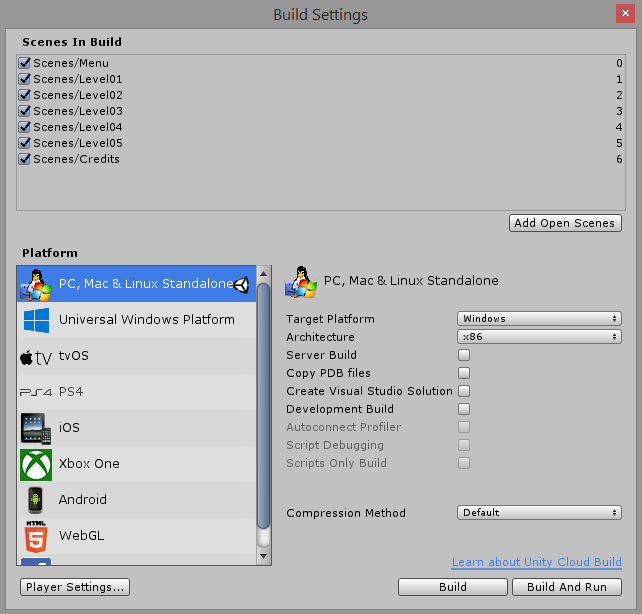
\includegraphics[width=.8\linewidth]{build.png}
  \caption{Okno Build pozwalające określić kolejność poziomów.}\label{rys_29}
  \begin{minipage}[t]{0.75\linewidth}
    \emph{Źródło: Opracowanie własne}
  \end{minipage}
\end{figure}


%%%%%%
\newpage
\section{Przygotowanie gry do publikacji}
\indent Gra jest już gotowa, jednakże nie jest stworzony żaden plik .exe, który będzie uruchamiał program. W oknie build, należy upewnić się, że wszystkie sceny są ustawione w prawidłowej kolejności. Następnie wymaganym jest wybranie platformy na którą chcemy stworzyć grę i potwierdzić przyciskiem Build. Pojawi się okienko w którym musimy wybrać katalog, w którym zostanie stworzona gra, która będzie skończonym produktem.

\indent W przypadku gdyby twórca chciał się podzielić grą z kimś znajomym, wystarczy ją spakować w .zip i wysłać. Aby produkt wyglądał na profesjonalny należy stworzyć plik instalacyjny. Do tworzenia małych plików instalacyjnych, idealnym narzędziem będzie Inno Setup. Jest to oprogramowanie służące do tworzenia plików instalacyjnych oparty na skryptach. Przez cały proces tworzenia pliku instalacyjnego prowadzi właśnie Inno, w jak najprostszy sposób, aby nie zmylić twórcy. W odpowiednim miejscu musimy wskazać ścieżkę do naszego pliku .exe, odpowiednio dla plików schowanych w folderze Data. 

\begin{figure}[!h]
\setcaptionwidth{1\linewidth}
\centering
  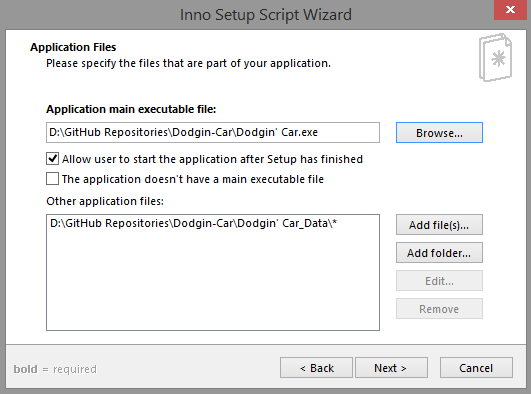
\includegraphics[width=0.7\linewidth]{inno.png}
  \caption{Okno wyboru ścieżki dostępu do pliku exe oraz folderu z danymi gry.}\label{rys_30}
  \begin{minipage}[t]{0.75\linewidth}
    \emph{Źródło: Opracowanie własne}
  \end{minipage}
\end{figure}

\end{quotation}
%%